%%%%%%%%%%%%%%%%%%%%%%%%%%%%%%%%%%%%%%%%%
% Jacobs Landscape Poster
% LaTeX Template
% Version 1.1 (14/06/14)
%
% Created by:
% Computational Physics and Biophysics Group, Jacobs University
% https://teamwork.jacobs-university.de:8443/confluence/display/CoPandBiG/LaTeX+Poster
% 
% Further modified by:
% Nathaniel Johnston (nathaniel@njohnston.ca)
%
% This template has been downloaded from:
% http://www.LaTeXTemplates.com
%
% License:
% CC BY-NC-SA 3.0 (http://creativecommons.org/licenses/by-nc-sa/3.0/)
%
%%%%%%%%%%%%%%%%%%%%%%%%%%%%%%%%%%%%%%%%%

%----------------------------------------------------------------------------------------
%	PACKAGES AND OTHER DOCUMENT CONFIGURATIONS
%----------------------------------------------------------------------------------------

\documentclass[final]{beamer}

\usepackage[scale=1.24]{beamerposter} % Use the beamerposter package for laying out the poster

\usetheme{confposter} % Use the confposter theme supplied with this template

\setbeamercolor{block title}{fg=ngreen,bg=white} % Colors of the block titles
\setbeamercolor{block body}{fg=black,bg=white} % Colors of the body of blocks
\setbeamercolor{block alerted title}{fg=white,bg=dblue!70} % Colors of the highlighted block titles
\setbeamercolor{block alerted body}{fg=black,bg=dblue!10} % Colors of the body of highlighted blocks
% Many more colors are available for use in beamerthemeconfposter.sty

%-----------------------------------------------------------
% Define the column widths and overall poster size
% To set effective sepwid, onecolwid and twocolwid values, first choose how many columns you want and how much separation you want between columns
% In this template, the separation width chosen is 0.024 of the paper width and a 4-column layout
% onecolwid should therefore be (1-(# of columns+1)*sepwid)/# of columns e.g. (1-(4+1)*0.024)/4 = 0.22
% Set twocolwid to be (2*onecolwid)+sepwid = 0.464
% Set threecolwid to be (3*onecolwid)+2*sepwid = 0.708

\newlength{\sepwid}
\newlength{\onecolwid}
\newlength{\twocolwid}
\newlength{\threecolwid}
\setlength{\paperwidth}{48in} % A0 width: 46.8in
\setlength{\paperheight}{36in} % A0 height: 33.1in
\setlength{\sepwid}{0.024\paperwidth} % Separation width (white space) between columns
\setlength{\onecolwid}{0.22\paperwidth} % Width of one column
\setlength{\twocolwid}{0.464\paperwidth} % Width of two columns
\setlength{\threecolwid}{0.708\paperwidth} % Width of three columns
\setlength{\topmargin}{-0.5in} % Reduce the top margin size
%-----------------------------------------------------------

\usepackage{graphicx}  % Required for including images

\usepackage{booktabs} % Top and bottom rules for tables

%----------------------------------------------------------------------------------------
%	TITLE SECTION 
%----------------------------------------------------------------------------------------

\title{PiFeed: Feed your pets with a Raspberry Pi} % Poster title

\author{Danny Duangphachanh, Daniel Friedman, Igor Janjic} % Author(s)

\institute{Bradley Department of Electrical and Computer Engineering, Virginia Tech [ECE 4564]} % Institution(s)

%----------------------------------------------------------------------------------------

\begin{document}

\addtobeamertemplate{block end}{}{\vspace*{2ex}} % White space under blocks
\addtobeamertemplate{block alerted end}{}{\vspace*{2ex}} % White space under highlighted (alert) blocks

\setlength{\belowcaptionskip}{2ex} % White space under figures
\setlength\belowdisplayshortskip{2ex} % White space under equations

\begin{frame}[t] % The whole poster is enclosed in one beamer frame

\begin{columns}[t] % The whole poster consists of three major columns, the second of which is split into two columns twice - the [t] option aligns each column's content to the top

\begin{column}{\sepwid}\end{column} % Empty spacer column

\begin{column}{\onecolwid} % The first column

%----------------------------------------------------------------------------------------
%	OBJECTIVES
%----------------------------------------------------------------------------------------

\begin{alertblock}{Objectives}

The purpose of PiFeed is to be able to remotely monitor and control a fish tank
and cat feeder from the internet. The ability to maintain a healthy
eating schedule for pets is a concern for members of our group, as well as many
others who travel or are away from home for an extended amount of time. By
euccessfully implementing a pet feeding and monitoring system using Raspberry
Pis, the stresses of animal care while away will be a thing of the past!
\begin{itemize}
    \item The system is composed of two Raspberry Pi's and one computer.
    \begin{itemize}
        \item Rasp1 collects information about the fish tank and controls the fish
        feeder.
        \item Rasp2 collects information about the cat and control the cat
        feeder.
    \end{itemize}
    \item A user will interface with the two Raspberry Pi's with a client
    application
    \begin{itemize}
        \item It is able to monitor both the aquarium and the cat feeder
        using Pi cameras.
        \item It also allows the user to customize the feeders and control them manually.
    \item We will consider the system successful if our pets can be fed
    remotely.
    \end{itemize}
\end{itemize}

\end{alertblock}

%----------------------------------------------------------------------------------------
%	INTRODUCTION
%----------------------------------------------------------------------------------------

\begin{block}{Introduction}

There are two Rasperry Pi's in this setup. RASPF1 is the Rasperry Pi that
controls the hardware for feeding for the fish tank. RASPC1 is the Rasperry Pi that
controls the hardware for feeding for the cat. PiFeed is separated into the
following modules: PiFeedControl, PiFeedFish, and PiFeedCat. The programming
language that was used to implement the feeding system is written in Python.
PiFeedControl is a program that is run on a client computer that has access to
the internet. It is used to remotely control the feeders using a custom socket
protocol. PiFeedFish is a program that is run on RASPF1 while PiFeedCat is a
program run on RASPC1. Each of these programs is responsible for controling the
camera, sensors, and feeder servos.

\end{block}



%----------------------------------------------------------------------------------------

\end{column} % End of the first column

\begin{column}{\sepwid}\end{column} % Empty spacer column

\begin{column}{\twocolwid} % Begin a column which is two columns wide (column 2)

\begin{columns}[t,totalwidth=\twocolwid] % Split up the two columns wide column

\begin{column}{\onecolwid}\vspace{-.6in} % The first column within column 2 (column 2.1)

%-------------------------------------------------------------------------------
% Materials
%%
\begin{block}{Hardware Description}
The following hardware was used to construct the feeding system:

\begin{itemize}
\item 2 Raspberry Pis
\item 2 SD cards
\item 2 WiFli + Bluetooth 3.0 USB adapters
\item 2 MicroUSB cables
\item 2 USB chargers
\item 2 5MP camera board modules
\item 1 Cheap LCD
\item 1 Servo
\item 1 Servo board
\item 1 H bridge
\item 1 DHT22 Temperature + Humidity sensor
\item Jumper wires
\end{itemize}

\end{block}

%----------------------------------------------------------------------------------------

\end{column} % End of column 2.1

\begin{column}{\onecolwid}\vspace{-.6in} % The second column within column 2 (column 2.2)

%----------------------------------------------------------------------------------------
%	METHODS
%----------------------------------------------------------------------------------------

\begin{block}{Methods}

    Methods

\end{block}

\begin{figure}
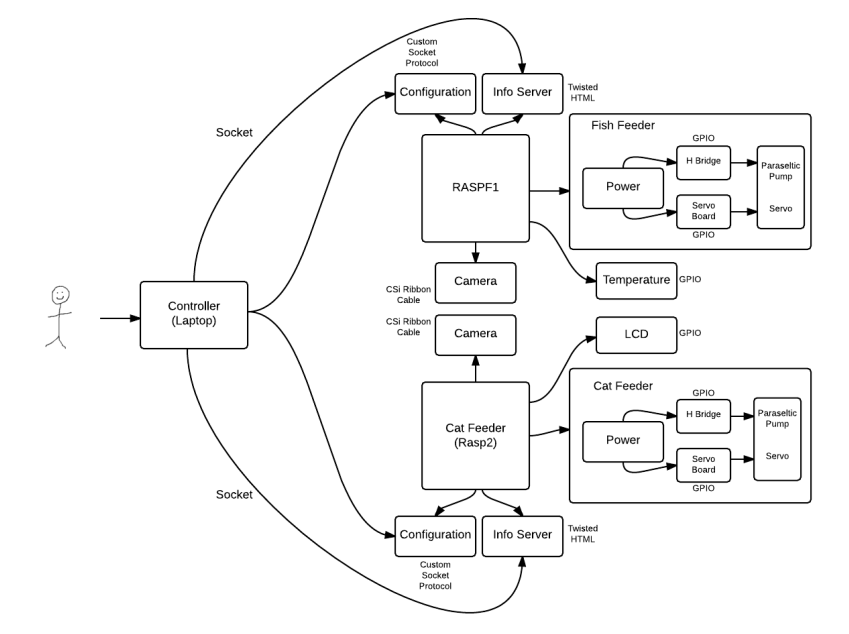
\includegraphics[width=1\linewidth]{UseCaseDiagram}
\caption{Use case diagram of the system.}
\end{figure}


%----------------------------------------------------------------------------------------

\end{column} % End of column 2.2

\end{columns} % End of the split of column 2 - any content after this will now take up 2 columns width

%----------------------------------------------------------------------------------------
%	IMPORTANT RESULT
%----------------------------------------------------------------------------------------

\begin{alertblock}{GitHub Page}
    \centering
----- \url{https://github.com/zergler/PiFeed} -----

\end{alertblock} 

%----------------------------------------------------------------------------------------

\begin{columns}[t,totalwidth=\twocolwid] % Split up the two columns wide column again

\begin{column}{\onecolwid} % The first column within column 2 (column 2.1)

%----------------------------------------------------------------------------------------
%	MATHEMATICAL SECTION
%----------------------------------------------------------------------------------------

\begin{block}{Testable Requirements}
A completely successful project should demonstrate that the following requirements are satisfied.
\begin{itemize}
    \item Able to feed the fish locally, remotely, manually and at specific times of the day.
    \item Able to feed the cat both locally, remotely, manually and at specific times of the day.
    \item Able to monitor the fish locally and remotely using the Pi camera.
    \item Able to monitor the cat locally and remotely using the Pi camera.
    \item Able to view the fish tank sensors locally and remotely.
    \item Able to view the cat sensors locally and remotely.
\end{itemize}

\end{block}

%----------------------------------------------------------------------------------------

\end{column} % End of column 2.1

\begin{column}{\onecolwid} % The second column within column 2 (column 2.2)

%----------------------------------------------------------------------------------------
%	RESULTS
%----------------------------------------------------------------------------------------

\begin{block}{Results}

\begin{figure}

\includegraphics[width=0.8\linewidth]{placeholder.jpg}
\caption{Figure caption}
\end{figure}

Nunc tempus venenatis facilisis. Curabitur suscipit consequat eros non porttitor. Sed a massa dolor, id ornare enim:

\begin{table}
\vspace{2ex}
\begin{tabular}{l l l}
\toprule
\textbf{Treatments} & \textbf{Response 1} & \textbf{Response 2}\\
\midrule
Treatment 1 & 0.0003262 & 0.562 \\
Treatment 2 & 0.0015681 & 0.910 \\
Treatment 3 & 0.0009271 & 0.296 \\
\bottomrule
\end{tabular}
\caption{Table caption}
\end{table}

\end{block}

%----------------------------------------------------------------------------------------

\end{column} % End of column 2.2

\end{columns} % End of the split of column 2

\end{column} % End of the second column

\begin{column}{\sepwid}\end{column} % Empty spacer column

\begin{column}{\onecolwid} % The third column

%----------------------------------------------------------------------------------------
%	CONCLUSION
%----------------------------------------------------------------------------------------

\begin{block}{Conclusion}

PiFeed is a system of connected Raspberry Pi units that allow the user to care
for their cat and/or fish locally and/or remotely. The PiFeed system is capable
of maintaining a feeding schedule and setting food for your pet cats and/or
fish. The PiFeed system also allows the user to manually control when a feeding
occurs by accessing the feeder via web service. Both the cat feeder and fish
feeder may be monitored through the use of a Raspberry Pi camera and may be seen
via web service. For the cat feeder, a sensor is used to detect the presence of
a cat and allows the distribution of food once detected.

\end{block}

%----------------------------------------------------------------------------------------
%	ADDITIONAL INFORMATION
%----------------------------------------------------------------------------------------

\begin{block}{Additional Information}

Maecenas ultricies feugiat velit non mattis. Fusce tempus arcu id ligula varius dictum. 
\begin{itemize}
\item Curabitur pellentesque dignissim
\item Eu facilisis est tempus quis
\item Duis porta consequat lorem
\end{itemize}

\end{block}

%----------------------------------------------------------------------------------------
%	REFERENCES
%----------------------------------------------------------------------------------------

\begin{block}{References}

\nocite{*} % Insert publications even if they are not cited in the poster
\small{\bibliographystyle{unsrt}
\bibliography{sample}\vspace{0.75in}}

\end{block}

%----------------------------------------------------------------------------------------
%	ACKNOWLEDGEMENTS
%----------------------------------------------------------------------------------------

\setbeamercolor{block title}{fg=red,bg=white} % Change the block title color

\begin{block}{Acknowledgements}

\small{\rmfamily{We would like to thank Dr. Plymale and Thaddeus Czauski for the interesting and challenging course.}} \\

\end{block}

%----------------------------------------------------------------------------------------
%	CONTACT INFORMATION
%----------------------------------------------------------------------------------------

\setbeamercolor{block alerted title}{fg=black,bg=norange} % Change the alert block title colors
\setbeamercolor{block alerted body}{fg=black,bg=white} % Change the alert block body colors

\begin{alertblock}{Contact Information}

\begin{itemize}
\item Danny Duangphachanh: \href{mailto:bboydd@vt.edu}{bboydd@vt.edu}
\item Daniel Friedman: \href{mailto:adfriedman@vt.edu}{adfriedman@vt.edu}
\item Igor Janjic: \href{mailto:ijanjic@vt.edu}{ijanjic@vt.edu}
\end{itemize}

\end{alertblock}

\begin{center}
\begin{tabular}{ccc}

\includegraphics[width=0.4\linewidth]{Logo} 
\end{tabular}
\end{center}

%----------------------------------------------------------------------------------------

\end{column} % End of the third column

\end{columns} % End of all the columns in the poster

\end{frame} % End of the enclosing frame

\end{document}
